\chapter{Introduction} 

In statistics, we work with collections of probability distributions, such as the normal, Poisson, and binomial distributions, to model random variables in various applications. These collections are known as \emph{statistical models}. Formally, a statistical model is defined as a set of probability distributions. In this thesis, we consider \emph{discrete statistical models} with \emph{finitely many state spaces} \( n + 1 \), which we view as subsets of the probability simplex \( \Delta_n \coloneqq \left\{ p \in \mathbb{R}^{n + 1} \mid \sum_{k=0}^n p_k = 1 \right\} \); a distribution \( p \in \Delta_n \) is a point in the probability simplex that assigns probabilities to the states \( 0, \dots, n \).
 
\begin{example}
Say we have a binomial random variable \( X \) with \( n + 1 \) states, then \( p = (p_k)_{k=0}^n = (\binom{n}{k} \theta^k (1-\theta)^{n-k})_{k=0}^n \) computes the probability of observing \( k \) successes in \( n \) trials with success probability \( \theta \in [0,1] \). The set \( \mathcal{M} = \left\{ (\binom{n}{k} \theta^k (1-\theta)^{n-k})_{k=0}^n \mid \theta \in [0,1] \right\} \) is our first example of a discrete statistical model, and it is known as the \emph{binomial model}.

\begin{figure}[H]
    \centering
    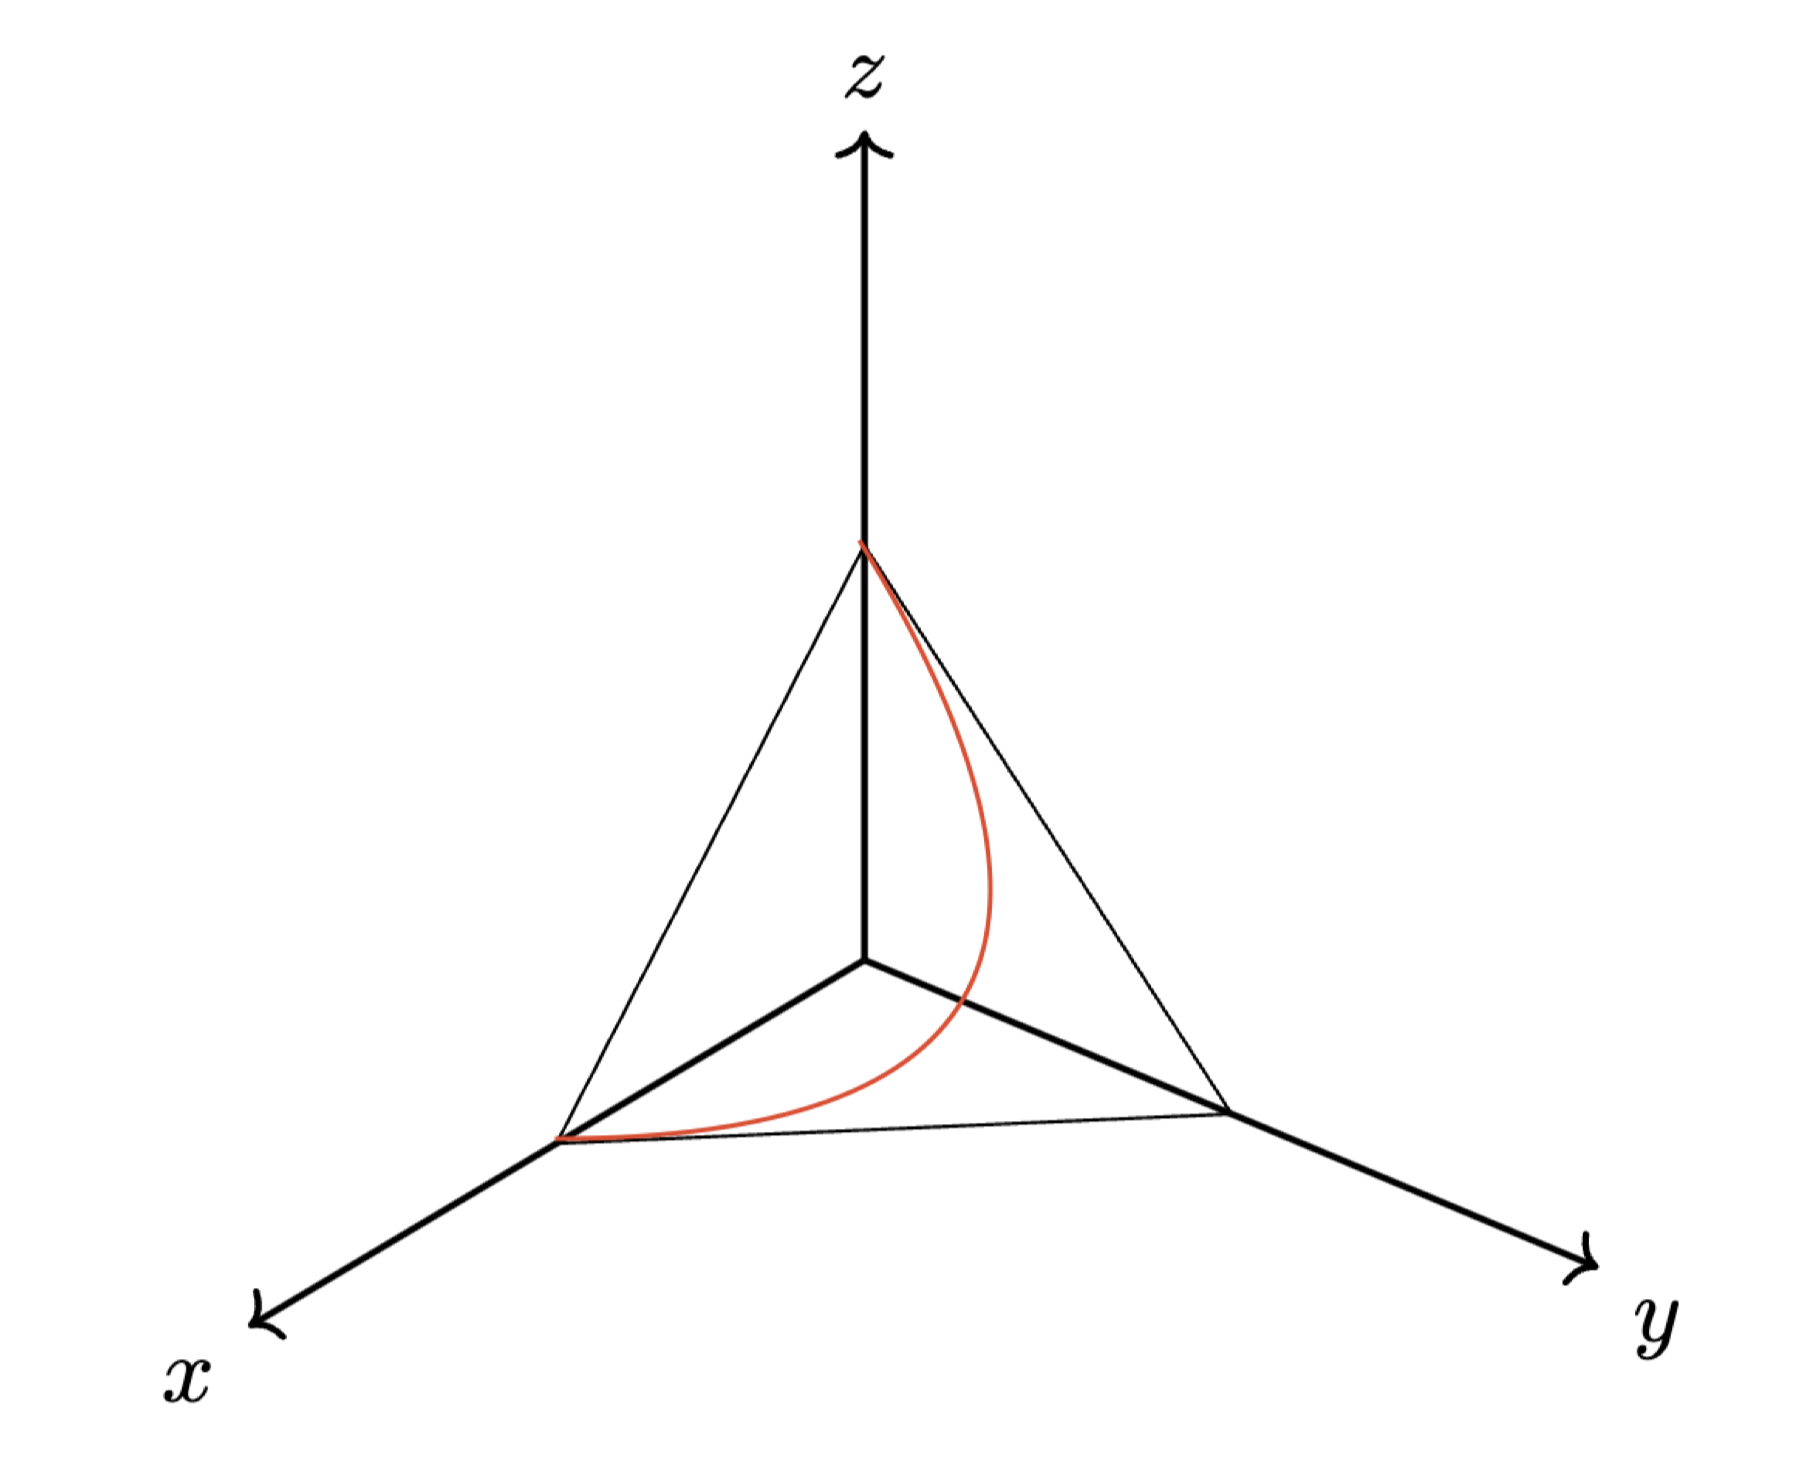
\includegraphics[width=0.43\textwidth]{assets/binom-discrete-model.png}
    \caption{This figure shows the probability simplex \( \Delta_2 \) with the binomial model (red curve). Every point on the curve is a binomial distribution.}
    \label{fig:binom-discrete-model}
\end{figure}
\end{example}

Given a statistical model \( \mathcal{M} \subset \Delta_n \) and data \( u \in \mathbb{N}^{n+1} \), a common problem in statistics is determining the distribution within a statistical model that best fits the data. ``Best'' can mean a lot of things; in \emph{maximum likelihood estimation}, it refers to finding the distribution that maximizes the probability of observing the data. The mapping \( \Phi: \Delta_n \to \mathcal{M}, u \mapsto \hat{p}\)
that assigns data \( u \) to a distribution \( \hat{p} \in \mathcal{M} \) in the best possible way, in the sense of maximum likelihood estimation, is called the \emph{maximum likelihood estimator (MLE)}. It is characterized by the property that \( \hat{p} \) maximizes for all \( p \in \mathcal{M} \) the log-likelihood function \( \ell(p) = \sum_{k=0}^n u_k \log p_k \).

We focus on \textbf{{one-dimensional {discrete} {statistical} {models} with rational MLE}}. These are models \( \mathcal{M} \) satisfying 
\begin{itemize}
    \item \( \mathcal{M} = \mathrm{image}(p) \) for some rational map \( p = (p_0, \dots, p_n): I \to \Delta_n \) where \( p_k \) is a rational map and \( I \subset \mathbb{R} \) is a union of closed intervals such that  \( p(\partial I) \subset \partial \Delta_n \), and
    \item all the \( n+1 \) coordinates of the MLE \( \Phi \) are rational functions in the data \( u \).
\end{itemize}

We ask two intriguing questions about these statistical models: (1) which \emph{form} do they take, and (2) can we \emph{classify} them, i.e. can we divide them into easier to understand models? June Huh gave an answer to the first question; he showed that if \( \Phi \) is rational, then each coordinate can be expressed as an alternating product of linear forms, where the numerator and denominator have the same degree \cite{huh2013varieties, huh2013maximum, duarte2021discrete}. For the second question, Arthur Bik and Orlando Marigliano provided a framework to classify discrete statistical models with rational MLE by introducing the concept of \emph{fundamental models} and \emph{chipsplitting games} \cite{bik2022classifying}.

This thesis builds upon the work of Bik and Marigliano. We present their findings on how fundamental models act as the building blocks of statistical models and investigate whether infinitely many fundamental models exist. It turns out that only finitely many fundamental models exist in \( \Delta_n \) for \( n \leq 4 \); a result that we will prove using the techniques by Bik and Marigliano. For \( n \geq 5 \), the problem remains open due to the complexity of the problem. This thesis advances the understanding of \( n = 5 \) by reducing the number of cases to check from 300,000 to 12,000. Furthermore, we present new findings on the number of fundamental models with a maximum degree of eleven in \( \Delta_6 \) and with a maximum degree of ten in \( \Delta_7 \). Moreover, we describe the algorithm for solving non-trivial hyperfield linear systems that underpins all the computational work discussed in this thesis. 

The chapters are organized as follows:
\begin{itemize}
    \item Chapter 2 provides tools to classify statistical models using fundamental models.
    \item Chapter 3 defines chipsplitting games and establishes the connection between fundamental statistical models and fundamental chipsplitting outcomes.
    \item Chapter 4 proves the finiteness of fundamental chipsplitting outcomes with positive support size \( n \leq 3 \) using the Invertibility Criterion.
    \item Chapter 5 shows the case \( n = 4 \) using the \emph{Hyperfield Criterion} and the Invertibility Criterion.
    \item Chapter 6 introduces the final tool, the \emph{Hexagon Criterion}, to show the case \( n = 5 \).
    \item Chapter 7 presents novel techniques to reduce the number of cases that need to be analyzed for \( n = 6 \).
    \item Chapter 8 computes the number of fundamental models.
    \item Chapter 9 concludes with a discussion on future research directions.
\end{itemize}


We could have opted to collect all the tools first and then apply them collectively to \( n \leq 5 \); however, we believe the current structure is more pedagogical as it emphasizes the challenges specific to each case.

The source code for the computations discussed in this thesis is available at \cite{ducrepo}.